% !TEX root = ../main.tex
\chapter{Introduction}

\label{ch:introduction}

Social media is...

\begin{itemize}
    \item
    A definition of social media in general
    \item
    Some examples of social media, including twitter, which I focus on in this thesis
    \item
    A graphic illustrating the differences between the aforementioned networks, also showing why twitter is best-suited for this
\end{itemize}

About 2 pages total for the introduction.

\pagebreak[2]

\chapter{Motivation}

\label{ch:motivation}

Social media is...

\begin{itemize}
    \item
    Big and growing
    \item
    Influencing people (e.g. election)
    \item
    Not used to its full potential by companies
\end{itemize}

About 2 pages total for the motivation part

\pagebreak[2]

\chapter{Background Theory}

\label{ch:backgroundTheory}

There is reason to believe companies would benefit from being able to analyze what their customers talk about (topics) and how they feel about these topics (sentiment by topic)

It could be used...
\begin{itemize}
    \item
    to monitor consumer sentiment
    \item
    to react to changes in sentiment in real-time (prevent and counteract "shitstorms")
    \item
    to use it as a feedback cycle for product development
\end{itemize}

About 1 page for the background theory

\pagebreak[1]

\iffalse
Below a few \LaTeX examples are included for beginners
\begin{figure}[ht]
    \centering
    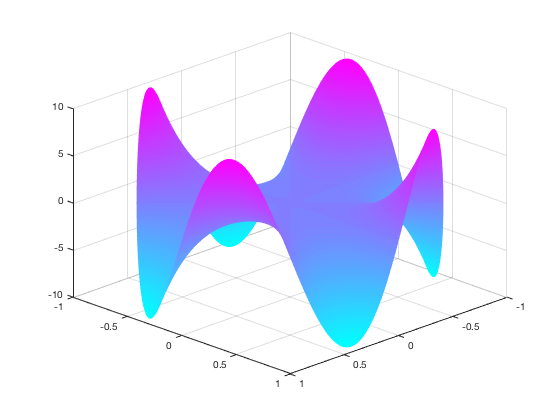
\includegraphics[width=5cm]{images/swing_function_plot.png}
    \caption{$u(x)$}%{Numerically solved solution}
    \label{fig:swingPlot}
\end{figure}


Equations can also be labeled
\begin{equation}
    \pi = \mathrm{e}^{i\cdot\phi}
    \label{eq:equation1}
\end{equation}


And later referenced. Even in subfigures.
\begin{figure}[!htb]
    \centering
    \begin{subfigure}[b]{0.3\textwidth}
        \centering
        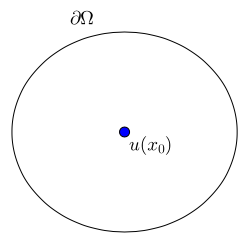
\includegraphics[width=\textwidth]{images/CircCenter}
        \caption{Equation \ref{eq:equation1}}\label{fig:circcenter}
    \end{subfigure}
    \hfill
    \begin{subfigure}[b]{0.3\textwidth}
        \centering
        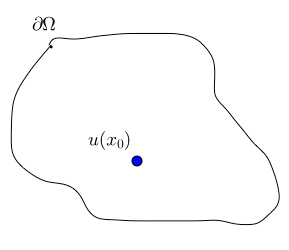
\includegraphics[width=\textwidth]{images/GeneralOffset}
        \label{fig:generaloffset}
        \caption{Equation \ref{eq:equation1}}
    \end{subfigure}
\end{figure}
\section{Including code}

Code can be using the package
\href{https://www.sharelatex.com/learn/Code\_Highlighting\_with\_minted}{Minted}.

An exaple of which of can be found below (see Source Code \ref{lst:nice_listing})
\begin{listing}
    %the language syntax can be declared here.
    \begin{minted}{python}
        import numpy as np

        def incmatrix(genl1,genl2):
        m = len(genl1)
        n = len(genl2)
        M = None #to become the incidence matrix
        VT = np.zeros((n*m,1), int)  #dummy variable

        #compute the bitwise xor matrix
        M1 = bitxormatrix(genl1)
        M2 = np.triu(bitxormatrix(genl2),1)

        for i in range(m-1):
        for j in range(i+1, m):
        [r,c] = np.where(M2 == M1[i,j])
        for k in range(len(r)):
        VT[(i)*n + r[k]] = 1;
        VT[(i)*n + c[k]] = 1;
        VT[(j)*n + r[k]] = 1;
        VT[(j)*n + c[k]] = 1;

        if M is None:
        M = np.copy(VT)
        else:
        M = np.concatenate((M, VT), 1)

        VT = np.zeros((n*m,1), int)

        return M
    \end{minted}

    \caption{My nice listing}
    \label{lst:nice_listing}
\end{listing}
\fi